\documentclass{article}

\usepackage[final]{neurips_2025}
\usepackage[utf8]{inputenc}
\usepackage[T1]{fontenc}
\usepackage{url}
\usepackage{booktabs}
\usepackage{siunitx}
\usepackage{graphicx}
\usepackage{amsmath}
\usepackage{microtype}
\usepackage[dvipsnames]{xcolor}
\usepackage{pgfplots}
\pgfplotsset{compat=1.18}
\makeatletter
\renewcommand{\@noticestring}{Conference on Physics and AI at Stanford University (PAI 2026).}
\makeatother

\definecolor{HumanBlue}{RGB}{42,120,189}
\definecolor{AIOrange}{RGB}{230,126,34}
\definecolor{GridGray}{RGB}{232,236,240}
\definecolor{AccentGreen}{RGB}{39,174,96}

\pgfplotsset{
  every axis/.append style={
    axis line style={black!70},
    tick style={black!60},
    ymajorgrids=true,
    grid style={GridGray},
    major grid style={line width=0.3pt},
    label style={font=\small},
    tick label style={font=\scriptsize},
    legend style={font=\scriptsize,draw=none,fill=none}
  }
}

\title{Epistemic Safety in AI Physics Tutors: Evaluating Pedagogical Structure in Generated Explanations}
\author{%
  Abdul Mohammad \\
  University of California, Berkeley \\
  \texttt{abdulmohammad@berkeley.edu}
}

\begin{document}
\maketitle

\begin{abstract}
AI systems often answer introductory physics questions correctly, yet students need explanations that expose the reasoning behind the answer. We frame this as an epistemic safety issue for AI tutoring: a fluent explanation can invite learner trust while omitting the conceptual bridge needed to detect misunderstanding. We study whether AI-generated explanations contain pedagogical discourse moves such as framing the physical situation, applying principles, checking conclusions, giving intuition-building examples, and marking caveats. Using 60 explanations across 20 introductory physics prompts, we compare human-written and AI-generated responses with sentence-level labels, quality ratings, and a lightweight keyword baseline. The annotation scheme reaches Cohen's $\kappa=0.6706$ on a 72-pair overlap subset. In this pilot, AI explanations match human explanations on correctness, show lower intuition-bridging coverage (20\% vs 35\%), and receive lower completeness ratings (4.0 vs 5.0). The findings suggest that AI physics tutor evaluation should treat explanation structure as a deployment check as well as a pedagogical preference.
\end{abstract}

\section{Introduction}
Evaluation at the intersection of physics and AI has advanced quickly, especially for answer-level reasoning tasks. Educational settings place an additional demand on these systems. A useful physics tutor needs to frame concepts, make reasoning legible, and connect formal equations to learner intuition. In practice, many LLM outputs are fluent and locally plausible while still being incomplete as teaching artifacts. This creates an epistemic safety concern: students can become confident in an explanation without having enough structure to notice what they do not understand.

Consider the question: why does an object moving in a circle accelerate even if its speed is constant? A thin answer may state that centripetal acceleration points inward. A stronger teaching explanation first addresses the misconception that constant speed implies no acceleration, explains that velocity includes direction, and then gives an intuitive example such as a car turning around a curve. Only the second exposes the reasoning a beginner needs to calibrate trust.

We treat this as a specific, limited form of AI safety for educational deployment. The risk is not physical harm or explicit hallucination. It is misplaced confidence caused by incomplete reasoning. When a response sounds coherent and authoritative, students may overtrust it even if key assumptions, caveats, or conceptual bridges are missing. The paper contributes:
\begin{itemize}
\item a compact 5-label discourse taxonomy with usable pilot reliability ($\kappa=0.6706$ on 72 overlap pairs),
\item a paired human and AI study showing lower AI intuition-bridging coverage at explanation level (-15 pp), and
\item a lightweight keyword baseline for sentence labeling, included to anchor the benchmark as a reproducible evaluation task.
\end{itemize}

\section{Related Work}
Recent benchmarks such as PhysReason and UGPhysics provide broad coverage of physics reasoning at answer level \citep{physreason2025,ugphysics2025}. The present study targets a narrower educational and safety-relevant question: whether a correct explanation contains the discourse moves that support calibrated understanding. Methodologically, the annotation protocol follows established reliability guidance in computational linguistics \citep{cohen1960,landis1977,artstein2008}, adapted to a compact pedagogy-oriented taxonomy. The contribution is a discourse-aware evaluation layer for introductory physics explanation quality and for educational deployment checks.

\section{Dataset and Annotation Protocol}
\subsection{Data Scope and Sources}
The study uses 20 prompts and 60 explanations (1 human + 2 AI per prompt), distributed across mechanics (8 prompts), electricity and magnetism (8), and thermo/energy (4). Human references come from public introductory physics resources licensed for reuse and were normalized into a comparable explanatory format \citep{openstaxlicense}.

\begin{table}[t]
\centering
\small
\begin{tabular}{lccc}
\toprule
Category & Prompts & Human & AI \\
\midrule
Mechanics & 8 & 8 & 16 \\
Electricity \& Magnetism & 8 & 8 & 16 \\
Thermo/Energy & 4 & 4 & 8 \\
\midrule
Total & 20 & 20 & 40 \\
\bottomrule
\end{tabular}
\caption{Pilot dataset composition.}
\label{tab:dataset}
\vspace{-0.6em}
\end{table}

\subsection{Annotation Schema}
Each sentence receives exactly one of five labels (Table~\ref{tab:labels}). During calibration, principle statements and direct applications were merged into a single \texttt{PRINCIPLE} category because annotators most often confused that boundary. Explanation-level ratings are 1\textendash 5 for clarity, correctness, and completeness.

\begin{table}[t]
\centering
\scriptsize
\begin{tabular}{lll}
\toprule
Label & Plain meaning & Example function \\
\midrule
\texttt{FRAME} & Sets up the situation & Constant speed differs from constant velocity. \\
\texttt{PRINCIPLE} & States or applies a rule & Acceleration is change in velocity over time. \\
\texttt{VERIFY} & Checks a conclusion & Without inward force, motion would be straight. \\
\texttt{INTUITION} & Gives an example or analogy & A car turning around a curve changes direction. \\
\texttt{CAVEAT} & Marks a condition or limit & This assumes air resistance is negligible. \\
\bottomrule
\end{tabular}
\caption{Plain-English label guide used to make the discourse scheme readable beyond NLP specialists.}
\label{tab:labels}
\vspace{-0.8em}
\end{table}

\subsection{Reliability Protocol}
A 72-pair overlap subset was independently labeled by two annotators for calibration. Final agreement is $\kappa=0.6706$ and $P_o=0.8333$, which is suitable for pilot benchmark analysis with transparent limitations.

\subsection{Heuristic Baseline}
As a simple baseline, a rule-based classifier assigns sentence labels from cue phrases, such as analogy markers for \texttt{INTUITION} and qualification markers for \texttt{CAVEAT}. On 381 singly labeled sentences, this baseline reaches 70.6\% accuracy and 0.575 macro-F1. Most errors collapse \texttt{VERIFY} and \texttt{CAVEAT} into \texttt{PRINCIPLE}, giving a lower-bound comparison for future automated labeling work.

\section{Results}
\subsection{Move Prevalence by Source}
Figure~\ref{fig:move-presence} shows explanation-level move presence rates. Both sources are saturated on \texttt{FRAME} and \texttt{PRINCIPLE} (100\%), then diverge on lower-frequency pedagogical moves. The strongest gap is \texttt{INTUITION} (35\% human vs 20\% AI), while AI shows higher \texttt{VERIFY} presence (75\% vs 65\%).

\begin{figure}[t]
\centering
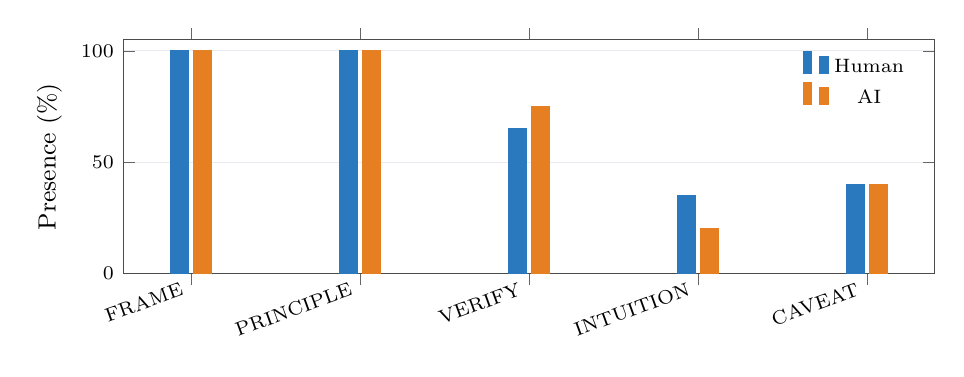
\begin{tikzpicture}
\begin{axis}[
    ybar,
    width=0.98\linewidth,
    height=4.55cm,
    bar width=6.4pt,
    ymin=0,ymax=105,
    ylabel={Presence (\%)},
    symbolic x coords={FRAME,PD,VERIFY,INTUITION,CAVEAT},
    xtick=data,
    xticklabels={FRAME,PRINCIPLE,VERIFY,INTUITION,CAVEAT},
    x tick label style={font=\scriptsize,rotate=20,anchor=east},
    legend style={at={(0.98,0.98)},anchor=north east},
]
\addplot+[fill=HumanBlue,draw=HumanBlue] coordinates {(FRAME,100) (PD,100) (VERIFY,65) (INTUITION,35) (CAVEAT,40)};
\addplot+[fill=AIOrange,draw=AIOrange] coordinates {(FRAME,100) (PD,100) (VERIFY,75) (INTUITION,20) (CAVEAT,40)};
\legend{Human,AI}
\end{axis}
\end{tikzpicture}
\caption{Explanation-level discourse move presence. AI responses show lower \texttt{INTUITION} prevalence despite matching human responses on \texttt{FRAME} and \texttt{PRINCIPLE}.}
\label{fig:move-presence}
\vspace{-0.9em}
\end{figure}

Sentence-level distributions are close on dominant structural content (\texttt{PRINCIPLE}: 55.37\% human, 54.62\% AI). The difference is concentrated in learner-facing bridges, with core inferential content remaining similar. This pattern is safety-relevant because introductory students often struggle to map a formal statement onto a physical situation. An explanation can be correct while still leaving that mapping implicit, creating a response that is trustworthy in surface form but weak as a guide to learner belief.

\subsection{Holistic Ratings}
Figure~\ref{fig:ratings} and Table~\ref{tab:ratings} summarize ratings from the primary annotator. Correctness is saturated (5.0 for both), while completeness shows the largest separation (5.0 human vs 4.0 AI).

\begin{figure}[t]
\centering
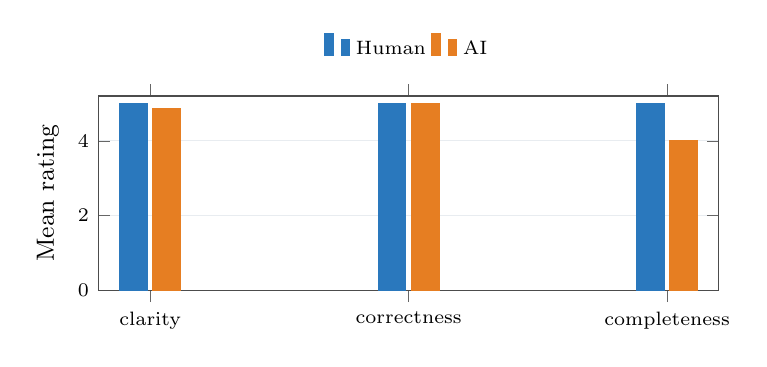
\begin{tikzpicture}
\begin{axis}[
    ybar,
    width=0.78\linewidth,
    height=4.05cm,
    bar width=10pt,
    ymin=0,ymax=5.2,
    ylabel={Mean rating},
    symbolic x coords={clarity,correctness,completeness},
    xtick=data,
    legend style={at={(0.5,1.13)},anchor=south,legend columns=2},
]
\addplot+[fill=HumanBlue,draw=HumanBlue] coordinates {(clarity,5.0) (correctness,5.0) (completeness,5.0)};
\addplot+[fill=AIOrange,draw=AIOrange] coordinates {(clarity,4.875) (correctness,5.0) (completeness,4.0)};
\legend{Human,AI}
\end{axis}
\end{tikzpicture}
\caption{Holistic ratings by source. Correctness is saturated; completeness carries the strongest separation signal.}
\label{fig:ratings}
\vspace{-0.9em}
\end{figure}

\begin{table}[t]
\centering
\small
\begin{tabular}{lccc}
\toprule
Source & Clarity & Correctness & Completeness \\
\midrule
Human ($n=20$) & 5.000 & 5.000 & 5.000 \\
AI ($n=40$) & 4.875 & 5.000 & 4.000 \\
AI - Human & -0.125 & 0.000 & -1.000 \\
\bottomrule
\end{tabular}
\caption{Mean holistic ratings.}
\label{tab:ratings}
\vspace{-0.8em}
\end{table}

\subsection{Uncertainty}
For key move contrasts, uncertainty remains wide at pilot scale: \texttt{INTUITION} difference is $-15.0$ pp (95\% CI: $[-39.3, 9.3]$, $p=0.206$) and \texttt{VERIFY} is $+10.0$ pp (95\% CI: $[-14.8, 34.8]$, $p=0.418$).
Prompt-level leave-one-out checks preserve the negative INTUITION direction ($[-21.1,-10.5]$ pp), although multiple-comparison-adjusted significance is not reached. We report this as directional pilot evidence. In qualitative review, the circular-motion examples show the same pattern: AI responses identify inward acceleration, while the human explanation more directly repairs the constant-speed misconception by distinguishing speed from velocity.

\section{Implications and Limitations}
The practical implication is that discourse labels can become a diagnostic layer for AI tutoring systems. A tutor response could be checked for correctness and then inspected for missing pedagogical moves: no physical framing, no everyday example, no stated idealization, or no misconception repair. A revision system could then ask the model to add the missing move. In a deployed tutor, this could function as a low-cost epistemic safety guardrail. The goal is to reduce fluent explanations that invite overtrust while leaving key reasoning steps hidden.

This is a pilot study. The dataset is small, interval estimates for move prevalence are wide, and aggregate ratings rely on one primary annotator. The human explanations were normalized for comparability, which reduces stylistic noise but may compress natural human variation. Completeness ratings also show no within-group variance in this summary, so inferential claims about that metric should remain cautious. The safety framing is also limited: the study does not measure overtrust directly, does not test downstream learning, and does not evaluate high-stakes physical action. The next version should use a larger multi-rater corpus, unrevised human sources, and learner-outcome validation.

\section{Conclusion}
This pilot study contributes a compact protocol for evaluating the pedagogical structure of AI-generated physics explanations. The evidence suggests that educational AI systems should be evaluated for correctness and for the reasoning structure that helps learners understand, question, and calibrate trust in an explanation. In that sense, explanation structure is part of epistemic safety for AI tutors.

\bibliographystyle{plainnat}
\bibliography{references}

\end{document}
